\section{Эйзенштейново тождество и точные ширины классических конструкций}
\label{sec:identity}

Метод применим и как <<измерительный инструмент>>: для каждой явной решёточной
конструкции из \cite{ABPR} можно вычислить точную ширину $d$ её запрещённого
интервала (в самой работе доказывалось лишь $d\ge1$). Добавим к ним
рациональные конструкции работы~\cite{Bounds}. Результаты для $4\le n\le9$
(каждая строка --- оценка $\chi(\R^n,[1,\ell])\le k$ при $\ell<d$; десятичные
значения $d$ округлены вниз):

\begin{center}\small
\resizebox{\textwidth}{!}{%
\begin{tabular}{c c l l l}
\toprule
$n$ & $k$ & решётка / конструкция & $d^2$ & $d$\\
\midrule
4 & 43   & эйзенштейнова решётка (\cite{Bounds}, теорема~2)
  & $^{\P}$ & $1{,}004110$\\
4 & 45   & $\Lambda_{45}$, общего положения (теорема~\ref{thm:main}) & $^{\dagger}$ & $1{,}016339$\\
4 & 48   & общего положения (теорема~\ref{thm:main}) & $^{\dagger}$ & $1{,}039657$\\
4 & 49   & $(3+\omega)D_4$ & $7/6$ & $1{,}080123$\\
4 & 54   & $A_4^*$ & $23/20$ & $1{,}072380$\\
5 & 132  & рациональная решётка общего положения (\cite{Bounds}, теорема~3)
  & $^{\dagger}$ & $1{,}010897$\\
5 & 140  & $A_5^*$, матрица $C_5$ из \cite{ABPR} & $39/35$ & $1{,}055597$\\
6 & 343  & $(3+\omega)E_6^*$ & $7/6$ & $1{,}080123$\\
7 & 1029 & ламинирование $E_6^*/343$ (\cite{Bounds}, теорема~4)
  & $^{\S}$ & $1{,}032878$\\
7 & 1323 & рациональная решётка общего положения
  (точный сертификат в полной версии~\cite{Full})
  & $^{\dagger}$ & $1{,}007032$\\
7 & 1372 & $E_7^*$, матрица $C_7$ из \cite{ABPR} & $17/14$ & $1{,}101946$\\
8 & 2401 & $(3+\omega)E_8$ & $7/6$ & $1{,}080123$\\
9 & 7203 & ламинирование $E_8/2401$ (\cite{Bounds}, теорема~5)
  & $^{\ddagger}$ & $1{,}016612$\\
9 & 17253& $A_9^*$, матрица $C_9$ из \cite{ABPR} & $169/165$ & $1{,}012048$\\
\bottomrule
\end{tabular}%
}

\smallskip
\begin{minipage}{0.92\textwidth}\footnotesize
$^{\dagger}$~точная дробь $d^2$ громоздка (числитель и знаменатель --- порядка
$30$ десятичных знаков): она равна отношению полей
\texttt{Ddown2}/\texttt{diamup2} файлов \path{audit-data/results/cert45.json}
и \path{audit-data/results/cert48.json} и отношению
\texttt{minimum\_distance\_squared}/\texttt{diameter\_squared} (блок
\texttt{separation}) сертификатов индексов $132$ и $1323$.\quad
$^{\S}$~$d^2=103332736237500000/96858928789031597$
(\path{audit-data/results/dim7_1029_exact.json}).\quad
$^{\ddagger}$~$d^2=1157058980000000/1119552292542693$
(\path{audit-data/results/dim9_7203_exact.json}).\quad
$^{\P}$~$d^2=298768283679964998359742207/296327113258585430253847000$
(\path{audit-data/results/dim4_k43_verify.json}).
\end{minipage}
\end{center}

Строки с $d^2=7/6$ --- это все эйзенштейновы конструкции индекса $7^{n/2}$, и
их ширина --- не совпадение, а тождество.

\subsection{Тождество для эйзенштейновых конструкций}
\label{ssec:eis}

Для решёток с $\Z[\omega]$-структурой ($\omega=e^{2\pi i/3}$) и подрешётки
$\Gamma=(3+\omega)\Lambda$ (умножение на $\alpha=3+\omega$, $|\alpha|^2=7$)
выполняется точное равенство
\begin{equation}\label{eq:eis}
D\bigl((3+\omega)\Lambda\bigr)^2=\tfrac73\,\lambda_1(\Lambda)^2,
\qquad\text{т.е.}\qquad
d=\frac{\sqrt{7/3}}{\,2R/\lambda_1\,},
\end{equation}
где $R$ --- радиус покрытия. Ширина $d$ зависит \emph{только} от отношения
покрытие/упаковка (рис.~\ref{fig:eis}): при $2R/\lambda_1=\sqrt2$ (решётки
$D_4$, $E_6^*$, $E_8$) получается ровно $d=\sqrt{7/6}$.

Обе половины~\eqref{eq:eis} доказываются ниже --- и сразу для всех
эйзенштейновых решёток, без перебора конкретных случаев. Оценка снизу
(предложение~\ref{prop:planar}) проектирует ячейку на плоскость минимального
вектора; оценка сверху (предложение~\ref{prop:eisup}) предъявляет в ячейке
явную точку.

\begin{proposition}[планарная нижняя граница]\label{prop:planar}
Пусть $\Lambda\subset\R^n$ --- решётка с $\Z[\omega]$-структурой.
Тогда для каждого ненулевого $w\in\Lambda$
\[
D\bigl((3+\omega)w\bigr)\ \ge\ \sqrt{7/3}\,\|w\|,
\qquad\text{в частности}\qquad
D\bigl((3+\omega)\Lambda\bigr)\ \ge\ \sqrt{7/3}\,\lambda_1(\Lambda).
\]
\end{proposition}

\begin{proof}
Векторы $\pm w,\ \pm\omega w,\ \pm(1+\omega)w$ лежат в $\Lambda$ и имеют одну
норму $\|w\|$ (умножение на обратимые элементы $\Z[\omega]$ --- изометрия
плоскости $P=\mathrm{span}(w,\omega w)$). Соответствующие шесть полупространств
$\langle x,u\rangle\le\|u\|^2/2$ содержат $V_0$, а их нормали лежат в $P$,
поэтому ортопроекция $\pi_P(V_0)$ содержится в правильном шестиугольнике $H$ ---
ячейке Вороного решётки $\Z[\omega]w\cong A_2$ масштаба $\|w\|$ внутри $P$.
Точка $v/2=(3+\omega)w/2$ лежит в $P$, и
\[
\dist\bigl(v/2,\,V_0\bigr)\ \ge\ \dist_P\bigl(v/2,\,H\bigr)
=\sqrt{7/12}\,\|w\|,
\]
где последнее равенство --- плоская выкладка в $A_2$: расстояние от точки
$(3+\omega)/2$ до шестиугольника с фасетами на расстоянии $1/2$ равно
$\sqrt{7/12}$ (та же выкладка даёт известную ширину $\sqrt7/2$ семицветной
раскраски $A_2/7$). Отсюда
$D(v)=2\dist(v/2,V_0)\ge\sqrt{7/3}\,\|w\|$.
\end{proof}

Обратное неравенство доказывается предъявлением в $V_0$ одной явной точки.
Технический приём выделим отдельно --- он понадобится ещё дважды.

\begin{lemma}[точка в ячейке]\label{lem:cellpoint}
Пусть $u_1,\dots,u_s$ --- минимальные векторы решётки $\Lambda$,
$q=\sum_i c_iu_i$ с $c_i\ge0$ и $\sum_ic_i\le1$. Если
$\langle q,u_j\rangle\le\frac12\lambda_1^2$ при всех $j$, то $q\in V_0$.
\end{lemma}

\begin{proof}
Ячейка задаётся опорными полупространствами: $x\in V_0$ равносильно
$\langle x,r\rangle\le\frac12\|r\|^2$ для всех $r\in\Lambda$ (это в точности
$\|x\|\le\|x-r\|$). Пусть $r\in\Lambda$. Для каждого $i$ с $r\ne u_i$ разность
$r-u_i$ --- ненулевой вектор решётки, поэтому
$\|r-u_i\|^2\ge\lambda_1^2=\|u_i\|^2$, откуда после раскрытия квадрата
\begin{equation}\label{eq:minhalf}
\langle r,u_i\rangle\ \le\ \tfrac12\|r\|^2 .
\end{equation}
Если $r\notin\{u_1,\dots,u_s\}$, то~\eqref{eq:minhalf} верно для всех $i$ и
$\langle q,r\rangle\le\bigl(\sum_ic_i\bigr)\frac12\|r\|^2\le\frac12\|r\|^2$
(здесь использовано $\frac12\|r\|^2\ge0$). Если же $r=u_j$, то нужное
неравенство --- это условие леммы. Случай $r=0$ тривиален.
\end{proof}

\begin{proposition}[верхняя граница]\label{prop:eisup}
Пусть $\Lambda$ --- решётка с $\Z[\omega]$-структурой и
$w\in\Lambda$ --- минимальный вектор. Тогда
\[
q=\tfrac13\bigl(2w+\omega w\bigr)\in V_0,
\qquad\text{и, как следствие,}\qquad
D\bigl((3+\omega)\Lambda\bigr)\ \le\ \sqrt{7/3}\,\lambda_1(\Lambda).
\]
\end{proposition}

\begin{proof}
Из $1+\omega+\omega^2=0$ следует $w+\omega w=-\omega^2w$, а умножение на
$\omega^2$ --- изометрия, поэтому $\|w+\omega w\|^2=\|w\|^2$. Раскрывая левую
часть и пользуясь $\|\omega w\|=\|w\|$, получаем
$2\|w\|^2+2\langle w,\omega w\rangle=\|w\|^2$, то есть
\begin{equation}\label{eq:eisip}
\langle w,\omega w\rangle=-\tfrac12\|w\|^2=-\tfrac12\lambda_1^2 .
\end{equation}
Векторы $w$ и $\omega w$ минимальны, $q=\frac23w+\frac13(\omega w)$ ---
выпуклая комбинация, и по~\eqref{eq:eisip}
\[
\langle q,w\rangle=\tfrac13\bigl(2\|w\|^2-\tfrac12\|w\|^2\bigr)=\tfrac12\lambda_1^2,
\qquad
\langle q,\omega w\rangle=\tfrac13\bigl(2\langle w,\omega w\rangle+\|\omega w\|^2\bigr)=0 .
\]
Лемма~\ref{lem:cellpoint} даёт $q\in V_0$. Положим $v=(3+\omega)w\ne0$. По
лемме~\ref{lem:mid} $D(v)=2\dist(v/2,V_0)\le2\|v/2-q\|$, причём
\[
\frac v2-q=\frac{3w+\omega w}2-\frac{2w+\omega w}3=\frac{5w+\omega w}6,
\qquad
\|5w+\omega w\|^2=\bigl(25+1-5\bigr)\|w\|^2=21\lambda_1^2
\]
(снова по~\eqref{eq:eisip}). Значит $\|v/2-q\|^2=\frac{21}{36}\lambda_1^2
=\frac7{12}\lambda_1^2$ и $D(v)^2\le\frac73\lambda_1^2$. Осталось заметить, что
$v$ --- ненулевой вектор подрешётки $(3+\omega)\Lambda$, а $D(\Gamma)$ ---
минимум по всем таким векторам.
\end{proof}

\begin{keybox}
\begin{theorem}[тождество для эйзенштейновых конструкций]\label{thm:eis}
Для любой решётки $\Lambda$ с $\Z[\omega]$-структурой выполнено
равенство~\eqref{eq:eis}:
$D\bigl((3+\omega)\Lambda\bigr)^2=\frac73\,\lambda_1(\Lambda)^2$, причём минимум
достигается ровно на образах минимальных векторов.
\end{theorem}
\end{keybox}

\begin{proof}
Предложения~\ref{prop:planar} и~\ref{prop:eisup}.
\end{proof}

Существенно, что предложение~\ref{prop:eisup} \emph{не} использует ни описания
граней $V_0$, ни предположения о том, что вороновски существенные векторы
минимальны: точка $q$ --- вершина шестиугольника $H$ из
предложения~\ref{prop:planar} (центроид треугольника $\{0,w,(1+\omega)w\}$,
$\|q\|=\lambda_1/\sqrt3$), и лемма~\ref{lem:cellpoint} говорит, что срезать эту
вершину нельзя ни у какой эйзенштейновой решётки. Проверка вида
<<вершину могли бы отсечь лишь векторы нормы $<\frac2{\sqrt3}\lambda_1$, а у
данной решётки таких нет>> становится излишней (ср.~\S\ref{ssec:prodneg}).

Тот же аргумент, применённый ко всем шести вершинам, описывает сечение ячейки
целиком.

\begin{corollary}[плоское сечение и точная $\alpha$-лестница]\label{cor:hexcell}
В обозначениях предложения~\ref{prop:planar}
$V_0\cap P=H$, и для любого $\alpha\in\Z[\omega]$
\[
D(\alpha\Lambda)\ =\ 2\,\lambda_1(\Lambda)\cdot\dist\bigl(\alpha/2,\ H_1\bigr),
\]
где $H_1$ --- ячейка Вороного $\Z[\omega]$ (правильный шестиугольник с фасетами
на расстоянии $1/2$). То есть неравенство $\alpha$-лестницы
(предложение~\ref{prop:alphaladder} ниже) для $\Z[\omega]$ --- на самом деле
равенство.
\end{corollary}

\begin{proof}
Шесть вершин $H$ --- это $\pm\omega^kq$, $k=0,1,2$, где $q$ построено
по минимальному вектору $\omega^kw$; каждая лежит в $V_0$ по
предложению~\ref{prop:eisup} (для $-\omega^kq$ применяем определение $V_0$
к $-r$). По выпуклости $H\subseteq V_0$, а включение $V_0\cap P\subseteq
\pi_P(V_0)\subseteq H$ доказано в предложении~\ref{prop:planar}; значит
$V_0\cap P=H$. Для $\alpha w/2\in P$ отсюда
$\dist(\alpha w/2,V_0)\le\dist(\alpha w/2,H)$, а $\pi_P(V_0)\subseteq H$ вместе
с $1$-липшицевостью проекции даёт обратное неравенство, так что
$D(\alpha w)=2\|w\|\dist(\alpha/2,H_1)$. Для произвольного ненулевого
$u\in\Lambda$ то же рассуждение о проекции (доказательство
предложения~\ref{prop:planar}, где $\alpha=3+\omega$ нигде не использовано)
даёт $D(\alpha u)\ge2\|u\|\dist(\alpha/2,H_1)\ge2\lambda_1\dist(\alpha/2,H_1)$,
поэтому минимум по $\alpha\Lambda\setminus\{0\}$ достигается на минимальных
векторах.
\end{proof}

\begin{remark}[что именно используется]\label{rem:a2tri}
Эйзенштейнова структура в предложении~\ref{prop:eisup} нужна лишь для того,
чтобы гарантировать пару \emph{минимальных} векторов $w,u$ с
$\langle w,u\rangle=-\frac12\lambda_1^2$ (годится $u=\omega w$); тогда и
$w+u$ минимален --- <<$A_2$-треугольник>> в графе минимальных векторов. Для
любой решётки с таким треугольником лемма~\ref{lem:cellpoint} даёт
$\frac13(2w+u)\in V_0$ и, как в следствии~\ref{cor:hexcell},
$V_0\cap P=H$; в частности
\[
D(3w+u)=\sqrt{7/3}\,\lambda_1,\qquad\|3w+u\|=\sqrt7\,\lambda_1 .
\]
Как экран это сильнее инрадиусной леммы~\ref{lem:inradius}, дающей для того же
вектора лишь $D\le(\sqrt7-1)\lambda_1=1{,}6458\lambda_1$: любая подрешётка,
содержащая вектор вида $3w+u$, имеет $d\le\sqrt{7/3}/\rho$. Проверено на
неэйзенштейновых $A_3,A_4,A_5,D_5,E_7$ (совпадение до $10^{-11}$).
\end{remark}

Теорема~\ref{thm:eis} переводит константу $D_{\min}=\sqrt7$ всех
конструкций $(3+\omega)$ --- $D_4/49$, $E_6^*/343$, $E_8/2401$ и
горизонтальный пол ламинирования из \S\ref{sec:lam} --- из численно
проверенного факта в теорему, причём в обе стороны --- и как гарантию, и как
потолок. Численные проверки сохранены как независимый контроль: повекторное
неравенство подтверждено на $26\,640$ векторах $E_8$, $2\,466$ векторах
$E_6^*$ и $18$ векторах $A_2$ с запасом $10^{-11}$
(\path{audit-data/results/planar_inradius_checks.json}), а само равенство ---
на $A_2$, $D_4$, $E_6^*$, $E_8$, растянутых суммах $A_2\oplus cA_2$ и случайных
косых эйзенштейновых решётках комплексного ранга $2$ и $3$, с полным перебором
подрешётки в доказуемо полном окне $\|v\|<D_*+2R$
(\path{audit-data/results/eisenstein_identity_checks.json}).

Подчеркнём, что сама пороговая константа $\sqrt{7/3}$ здесь не нова: в
замечании~9 работы \cite{ABPR} отмечено, что их теорема~8 остаётся верной при
ослабленном условии $2R/\lambda_1\le\sqrt{7/3}\approx1{,}5275$ вместо $3/2$,
но авторы <<не знают решёток, которые использовали бы это усиление>>. Условие
$d\ge1$ в~\eqref{eq:eis} --- это в точности их ослабленное условие; новизна
здесь в другом: равенство~\eqref{eq:eis} даёт не только порог, но и \emph{точную}
ширину интервала для каждой конкретной решётки, а таблица выше как раз и
предъявляет решётки, реализующие усиление.

У решётки Лича $\Lambda_{24}$ отношение $2R/\lambda_1$ также равно $\sqrt2$, и
классическая оценка $\chi(\R^{24})\le7^{12}$ уже доказана в \cite{ABPR}
(там $7^{n/2}$ получено для $n\in\{6,8,24\}$). Теорема~\ref{thm:eis} добавляет
к ней \emph{точную ширину}:
\[
\chi\bigl(\R^{24},[1,\ell]\bigr)\le7^{12}\qquad(\ell<\sqrt{7/6}\,),
\]
и $\sqrt{7/6}$ здесь не улучшить в пределах этой конструкции --- верхняя
половина тождества запрещает. Для решётки Коксетера--Тодда $K_{12}$ имеем
$2R/\lambda_1=\sqrt{8/3}\approx1{,}633>\sqrt{7/3}$, и~\eqref{eq:eis} даёт
$d=\sqrt{7/8}\approx0{,}935<1$: конструкция теоремы~8 из \cite{ABPR} на
$K_{12}$ не проходит даже в усиленной форме замечания~9 (частичный
отрицательный ответ на их открытый вопрос~2). Подчеркнём, что этот вывод
опирается именно на верхнюю половину~\eqref{eq:eis}: с одной лишь нижней
границей оставался бы шанс, что настоящее $D(K_{12})$ больше планарного пола
(перебор $85\,680$ векторов в \S\ref{ssec:prodneg} закрывал этот шанс
вычислением, теперь он закрыт теоремой). В \S\ref{ssec:prodneg} тот же вывод
получен и для комплексного ранга~$5$ (размерность~$10$), где ни кодовая
конструкция ($2R/\lambda_1\approx1{,}826$), ни поиск по эрмитовым формам
($2R/\lambda_1\ge1{,}7496$) не опускаются ниже $\sqrt{7/3}$.

\begin{figure}[t]
\centering
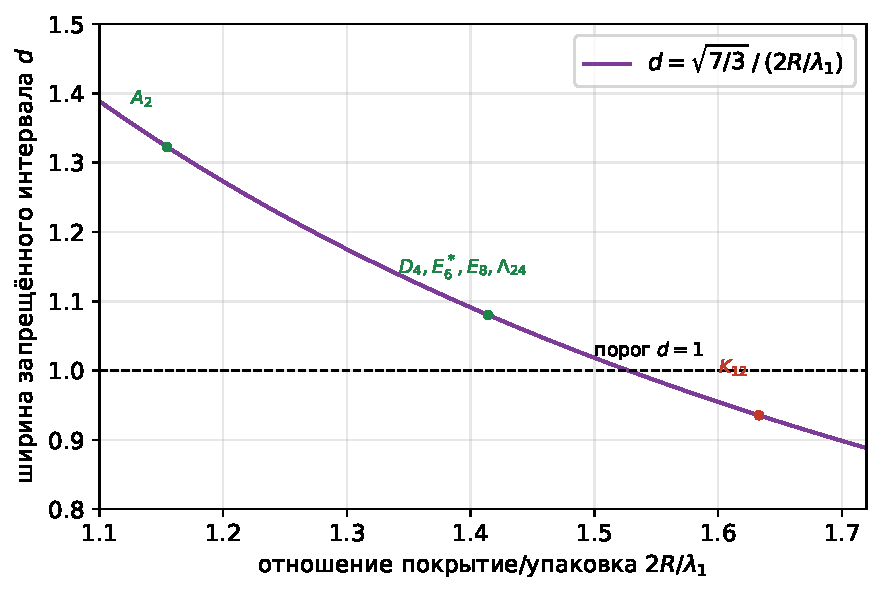
\includegraphics[width=0.6\textwidth]{fig_eisenstein.pdf}
\caption{Тождество~\eqref{eq:eis}: ширина $d$ эйзенштейновой конструкции против
отношения покрытие/упаковка $2R/\lambda_1$. По теореме~\ref{thm:eis} прямая
$d=\sqrt{7/3}/\rho$ --- не оценка, а точное значение для любой эйзенштейновой
решётки: $D_4,E_6^*,E_8$ (все с $\rho=\sqrt2$) дают ровно $d=\sqrt{7/6}$,
столько же --- $\Lambda_{24}$, а $K_{12}$ ($\rho=\sqrt{8/3}$) падает ниже
порога $d=1$.}
\label{fig:eis}
\end{figure}

\paragraph{Оптимальность конструкции $C_5$ на фиксированной $A_5^*$.}
Исчерпывающим перебором \emph{всех} $1\,424\,115\,231$ подрешёток
индекса~$140$ решётки $A_5^*$ установлено, что явная конструкция $C_5$ из
\cite{ABPR} оптимальна на этом индексе и по ширине:
$\max d=\sqrt{39/35}$. Оценка $\chi(\R^5)\le132$ работы~\cite{Bounds} этому
не противоречит: она меняет родительскую форму и использует индекс~$132$.

\subsection{\texorpdfstring{$\alpha$}{alpha}-лестница}
\label{ssec:alphaladder}

Чтобы продуктовое правило (предложение~\ref{prop:product}) было применимо,
для каждой размерности нужна лестница пар $(k,d)$. Одно семейство даёт её в
замкнутой форме сразу для всех порядков, действующих подобиями.

\begin{proposition}[$\alpha$-лестница]\label{prop:alphaladder}
Пусть $\mathcal R\in\{\Z,\Z[i],\Z[\omega],\mathcal H\}$ ($\mathcal H$ ---
кватернионы Гурвица), $\Lambda\subset\R^n$ --- модуль над $\mathcal R$, и
$\alpha\in\mathcal R$. Тогда $\Gamma=\alpha\Lambda$ имеет индекс $|\alpha|^n$ и
\[
D(\alpha w)\ \ge\ 2\,|w|\cdot\dist\bigl(\alpha/2,\ U\bigr)\quad\text{для всех }w\in\Lambda,
\]
где $U$ --- ячейка Вороного решётки $\mathcal R w$ при $|w|=1$: отрезок, квадрат,
шестиугольник или 24-ячейка. Как следствие
$d\ge 2\dist(\alpha/2,U)/\rho$, $\rho=\diam V_0/\lambda_1$.
Для минимального $w$ здесь на самом деле \emph{равенство} (следствие~\ref{cor:Uexact}).
\end{proposition}

Доказательство дословно повторяет планарную границу
(предложение~\ref{prop:planar}): единицы $\mathcal R$ дают равнонормные векторы
$uw$, чьи опорные полупространства лежат \emph{внутри} линейной оболочки
$\mathcal R w$, поэтому проекция $V_0$ на неё содержится в $U$, а расстояние
считается уже в этой оболочке.

Обратное включение $U\subseteq V_0$ --- это лемма~\ref{lem:cellpoint},
применённая к вершинам $U$; для каждого из четырёх порядков вершины
предъявляются явно.

\begin{corollary}[$\alpha$-лестница точна]\label{cor:Uexact}
Пусть $w$ --- минимальный вектор $\Lambda$, а $U_w$ --- ячейка
Вороного решётки $\mathcal Rw$ внутри $S=\mathrm{span}(\mathcal Rw)$ (то есть
$U$ в масштабе $\lambda_1$). Тогда $U_w=V_0\cap S$ и
\[
D(\alpha\Lambda)\ =\ 2\,\lambda_1(\Lambda)\cdot\dist\bigl(\alpha/2,\ U\bigr)
\qquad\text{для всех }\alpha\in\mathcal R .
\]
\end{corollary}

\begin{proof}
Все векторы $uw$ ($u$ --- единица $\mathcal R$) минимальны в $\Lambda$, так как
$|uw|=|w|=\lambda_1$. Каждая вершина $q$ многогранника $U_w$ --- выпуклая
комбинация таких векторов, для которой $\langle q,uw\rangle\le\frac12\lambda_1^2$
на участвующих:
\begin{itemize}[leftmargin=1.4em,itemsep=1pt]
\item отрезок ($\mathcal R=\Z$): $q=\frac12w$, сумма коэффициентов $\frac12$,
$\langle q,w\rangle=\frac12\lambda_1^2$;
\item квадрат ($\Z[i]$): $q=\frac12(w\pm iw)$, и $\langle q,w\rangle=
\langle q,\pm iw\rangle=\frac12\lambda_1^2$, так как $w\perp iw$;
\item шестиугольник ($\Z[\omega]$): $q=\frac13(2w+\omega w)$ ---
предложение~\ref{prop:eisup} ($\langle q,w\rangle=\frac12\lambda_1^2$,
$\langle q,\omega w\rangle=0$);
\item $24$-ячейка ($\mathcal H$): все $24$ вершины имеют вид
$\frac12(u_1+u_2)w$ с ортогональными единицами $u_1\perp u_2$ (например
$\frac12(1+i)w$) --- прямая проверка по списку $24$ единиц Гурвица; тогда
$\langle q,u_mw\rangle=\frac12\lambda_1^2$.
\end{itemize}
По лемме~\ref{lem:cellpoint} вершины лежат в $V_0$, а с ними по выпуклости и
весь $U_w$; обратное включение $V_0\cap S\subseteq\pi_S(V_0)\subseteq U_w$ ---
это доказательство предложения~\ref{prop:alphaladder}. Дальше --- дословно
доказательство следствия~\ref{cor:hexcell}: расстояние от точки $\alpha w/2\in S$
до $V_0$ зажато между $\dist(\alpha w/2,U_w)$ сверху и снизу, а по
предложению~\ref{prop:alphaladder} минимум по $\alpha\Lambda\setminus\{0\}$
достигается на минимальных векторах.
\end{proof}

Вещественный множитель даёт $\dist(m/2,[-1/2,1/2])=(m-1)/2$, то есть
$d=(m-1)/\rho$ --- это в точности предложение~\ref{prop:mult} ниже; эйзенштейнов
$3+\omega$ даёт $\sqrt{7/12}$, то есть $d=\sqrt{7/3}/\rho$. По
следствию~\ref{cor:Uexact} все эти значения --- точные, а не оценки снизу.
Отметим совпадение: кватернион Гурвица нормы~7, например $2+i+j+k$, даёт
\emph{ровно ту же} константу $\sqrt{7/12}$, а норма~8 (элемент $2+2i$) ---
константу $\sqrt{1/2}$, то есть требует $\rho\le\sqrt2$ при индексе
$8^{n/2}=2{,}828^n$. Равенство проверено численно для всех четырёх порядков
(\path{audit-data/results/eisenstein_identity_checks.json}).

\subsection{Вещественный множитель и инрадиусная лемма}
\label{ssec:mult}

Для $\Gamma=m\Lambda$ (индекс $m^n$) минимум $D$ достигается на $mu$ с
минимальным~$u$: минимальные векторы всегда релевантны по Вороному, поэтому
ячейка доходит ровно до $\lambda_1/2$ в этом направлении и
$\dist(mu/2,V_0)=(m-1)\lambda_1/2$.

\begin{proposition}\label{prop:mult}
$D_{\min}(m\Lambda)=(m-1)\lambda_1$, следовательно
$d=(m-1)/\rho$, где $\rho=\diam V_0/\lambda_1$. При $m=3$ это $d=2/\rho$, и
условие правильности --- ровно $\rho\le2$; при $m=2$ потребовалось бы
$\rho\le1$, что невозможно выше размерности~$1$.
\end{proposition}

\begin{proof}
Нижняя граница: для любого ненулевого $w\in\Lambda$ ячейка лежит в
полупространстве $\langle x,w\rangle\le\|w\|^2/2$, поэтому
\[
\dist\Bigl(\frac{mw}2,\,V_0\Bigr)\ \ge\
\frac{\langle mw/2,\,w\rangle-\|w\|^2/2}{\|w\|}
=\frac{(m-1)\|w\|}2\ \ge\ \frac{(m-1)\lambda_1}2.
\]
Верхняя: для минимального $u$ точка $u/2$ лежит на границе $V_0$, значит,
$\dist(mu/2,V_0)\le\|mu/2-u/2\|=(m-1)\lambda_1/2$. Вместе это равенство.
\end{proof}

Правило $d=2/\rho$ дополнительно сверено с прямым измерением на двенадцати
решётках, совпадение до шести знаков. Подчеркнём, что оно специфично для
\emph{вещественных} множителей: у $3+\omega$ минимум достигается в другом
месте, и там работает тождество~\eqref{eq:eis}. Обе формулы --- частные случаи
одного точного правила (следствие~\ref{cor:Uexact}): $\dist(\alpha/2,U)$ для
отрезка и для шестиугольника соответственно.

Тот же одностроч\-ный приём --- вписанный шар вместо опорного полупространства
--- даёт \emph{верхнюю} границу разделения, которая закрывает целый класс
поисков.

\begin{lemma}[инрадиусная граница]\label{lem:inradius}
Для любого $v$ с $\|v\|\ge\lambda_1$ выполнено
$D(v)\le\|v\|-\lambda_1$.
\end{lemma}

\begin{proof}
Шар $B(0,\lambda_1/2)$ содержится в $V_0$ (упаковочный радиус равен инрадиусу
ячейки), поэтому $\dist(v/2,V_0)\le\dist\bigl(v/2,B(0,\lambda_1/2)\bigr)
=\|v\|/2-\lambda_1/2$.
\end{proof}

\begin{corollary}\label{cor:no-subgroup}
Пусть $\rho<2$ (то есть раскраска $\Gamma=3\Lambda$ правильна с
запасом). Тогда никакая подрешётка $\Gamma'$ с
$3\Lambda\subsetneq\Gamma'\subseteq\Lambda$ не задаёт правильной раскраски:
индекс $3^n$ нельзя понизить, оставаясь над $3\Lambda$.
\end{corollary}

\begin{proof}
Такая $\Gamma'$ содержит ненулевой класс $c\in\Lambda/3\Lambda$; класс имеет
представитель $v$ нормы $\le R(3\Lambda)=3R$. По лемме~\ref{lem:inradius}
$D(v)\le3R-\lambda_1<2R=\diam V_0$ --- ровно потому, что $\rho<2$ означает
$R<\lambda_1$.
\end{proof}

Следствие~\ref{cor:no-subgroup} делает излишним исчерпывающий перебор
ненулевых классов $\Lambda/3\Lambda$ в поисках промежуточной подгруппы: в любой
размерности и для любой решётки с $\rho<2$ такой перебор не может дать ни
одного выжившего.

\subsection{Размерность 12: решётка Коксетера--Тодда вместо башни}
\label{ssec:k12}

Правило $d=2/\rho$ немедленно вознаграждает лучшую решётку. У решётки
Коксетера--Тодда $K_{12}$ отношение $\rho=2R/\lambda_1=\sqrt{8/3}$ известно
точно, поэтому
\[
\chi\bigl(\R^{12},[1,\ell]\bigr)\ \le\ 3^{12}
\qquad\Bigl(\ell<2\big/\sqrt{8/3}=\sqrt{3/2}=1{,}224745\Bigr)
\]
--- тот же индекс $531\,441$, что у классической оценки $3^n$
Лармана--Роджерса и у башни ламинаций $E_8$ (\S\ref{ssec:tower}), но ширина
$1{,}2247$ вместо численных $1{,}0755$ башни. Забавным образом $K_{12}$,
отвергнутая эйзенштейновым путём ($\rho>\sqrt{7/3}$, см.\ выше), оказывается
лучшим \emph{вещественным} носителем. Проверка: $K_{12}$ построена из гексакода
($[6,3,4]$ над $\mathbb F_4=\Z[\omega]/2$), $\lambda_1^2=4$ --- в точной целой
арифметике по всем $756$ минимальным векторам, $\det(\mathrm{Gram})=3^6$
точно, измеренный снизу радиус покрытия совпадает с точным $\sqrt{8/3}$ до
девятого знака, а $D_{\min}(3K_{12})=2\lambda_1$ --- по
предложению~\ref{prop:mult} и контрольному перечислению
(\path{audit-data/results/dim12_k12.json}).
